\documentclass[12pt,twocolumn]{article}
\usepackage[margin=2.0cm]{geometry}
\usepackage{amsmath,amssymb,graphicx,booktabs,siunitx}
\usepackage{url}
\usepackage[hidelinks]{hyperref}
\usepackage{caption}
\usepackage{microtype}
\sisetup{round-mode=places,round-precision=3}
\title{Scaling Relations in Fractional Gaussian Noise and Brownian Motion: A Finite-Sample Study}
\author{Braulio A. Ronquillo Nuñez\\}
\date{}
\begin{document}
\maketitle
\begin{abstract}
We compare scaling estimators for fractional Gaussian noise (fGn), its fractional Brownian motion (fBm) integral, and processes designed to disturb self-affine scaling. The distinction between stationary increment correlations and local path roughness controls which exponent identities are meaningful. Gaussian circulant embedding and Fourier synthesis provide two reference generators. We evaluate detrended fluctuation analysis (DFA), rescaled range, structure functions, autocorrelation, aggregated variance, spectral estimators, wavelets, and graph-dimension estimators across nine Hurst parameters, four lengths, and 200 realizations per configuration. Paired relation residuals receive unadjusted bootstrap intervals and multiplicity-corrected hypothesis tests. The finite-sample results show estimator-specific bias and clarify when apparent relation failures reflect fitting range, contaminated signals, or an inapplicable process definition.


\end{abstract}

\section{Introduction}

Several exponents are used to describe scale dependence in time series. The Hurst parameter $H$ is attached to increment scaling of a self-similar path, a spectral slope measures power near low frequency, and graph dimension describes local roughness. These quantities are linked for fractional Brownian motion (fBm) and its stationary increments, fractional Gaussian noise (fGn), but the identities require care about which process is being measured. An empirically fitted exponent can also depend strongly on the finite range of scales, the estimator and the presence of trends. The aim here is to test the identities numerically while keeping the process and measurement conventions explicit.

Mandelbrot and Van Ness introduced fBm and fractional noises as models of scale-dependent random variation \cite{mandelbrot1968}. Peng and colleagues developed detrended fluctuation analysis (DFA) for identifying correlation in heterogeneous sequences through an integrated profile and local trend removal \cite{peng1994}. The subsequent MF-DFA extension defines a family of fluctuation moments and recovers ordinary DFA at moment order two \cite{kantelhardt2002}. We use only the latter case because the present questions concern a single scaling exponent rather than a multifractal spectrum. Chen et al. show that nonstationarities and antipersistent data can produce DFA crossovers or finite-scale bias \cite{chen2002}. These methods thus complement, but do not replace, an explicit model for the signal.

The central conceptual issue is that long-lag dependence and short-lag roughness are different properties. Gneiting and Schlather construct covariance families that can control the two independently \cite{gneiting2004}. Accordingly, agreement between a dimension relation and a long-memory relation is evidence consistent with self-affinity over the observed scales; it is not a general mathematical consequence of either measurement alone. Our experiment includes a generalized Cauchy covariance to expose this distinction, as well as additive noise, a trend, a periodic component and a spectral cutoff.

\section{Theoretical background}
\subsection{fGn, fBm and covariance tails}

We normalize fBm $B_H(t)$ so that $B_H(0)=0$ and
\begin{equation}
 \mathrm{Var}[B_H(t+\tau)-B_H(t)]=|\tau|^{2H},\qquad 0<H<1.
 \label{eq:increment}
\end{equation}
Its unit increments $X_k=B_H(k+1)-B_H(k)$ are stationary Gaussian fGn, with covariance
\begin{equation}
 \gamma_H(k)=\frac{|k+1|^{2H}-2|k|^{2H}+|k-1|^{2H}}{2}.
 \label{eq:covariance}
\end{equation}
A second-order expansion at large $k$ gives $\gamma_H(k)\sim H(2H-1)k^{2H-2}$. For $H>1/2$, the coefficient is positive and the decay exponent in $C(k)\sim k^{-\beta}$ is $\beta=2-2H\in(0,1)$; the positive tail is not summable. For $H<1/2$, it is negative and $\beta>1$, so the tail is absolutely summable. This last case is antipersistent but not long-range dependent in the non-summable positive-covariance sense. At $H=1/2$ the nonzero-lag fGn covariance vanishes. Consequently, a log regression on \emph{positive} ACF values is defined only for the persistent portion of the grid. These identities follow directly from Eq.~\eqref{eq:covariance}; the original problem statement reverses the summability claim for $H<1/2$.

For a stationary fGn, the low-frequency spectral density behaves as
\begin{equation}
 S_X(f)\sim |f|^{-\alpha_g},\qquad \alpha_g=2H-1=1-\beta.
 \label{eq:spectrum}
\end{equation}
At $H<1/2$, $\alpha_g<0$ and the density tends to zero at the origin. Equation~\eqref{eq:spectrum} is a low-frequency asymptotic statement, not a guarantee of a single slope at all finite frequencies. Accumulation into a path multiplies the discrete Fourier transform by an approximate $f^{-1}$ factor away from zero. The finite-record fBm slope is therefore $\alpha_B=\alpha_g+2=2H+1$. The fBm path is nonstationary, so $\alpha_B$ is an operational Fourier exponent rather than a Wiener--Khinchin spectral density exponent of a stationary process.

The spectral relation can be seen more precisely from the covariance transform. When $0<\beta<1$, the positive long-lag tail has a non-integrable cosine transform as frequency tends to zero. In the continuous approximation,
\begin{equation}
\begin{aligned}
\int_0^\infty k^{-\beta}\cos(2\pi f k)\,dk
&=\Gamma(1-\beta)\sin\left(\frac{\pi\beta}{2}\right)\\
&\quad\times(2\pi f)^{\beta-1}.
\end{aligned}
\label{eq:cosine}
\end{equation}
The exponent of $f$ is $\beta-1$, which yields $\alpha_g=1-\beta$. This argument requires $0<\beta<1$ and a positive non-summable covariance tail. It cannot be copied verbatim to the antipersistent case, where $\beta>1$ and the integral's small-lag behavior is different. For fGn with $H<1/2$, however, the sum of the full covariance sequence is zero and the constant spectral term cancels; its exact covariance still gives $S_X(f)\propto|f|^{1-2H}$ near zero. Thus the algebraic equality $\alpha_g=1-\beta$ survives for this particular model while the usual positive-tail long-memory derivation does not. This distinction matters when an empirical negative ACF tail is fitted with a procedure intended for positive correlations.

The graph of fBm has dimension $D=2-H$, so for the path analyzed here the combined relations are
\begin{equation}
 D=\frac{5-\alpha_B}{2}=1+\frac{\beta}{2}.
 \label{eq:dimension}
\end{equation}
Here $\beta$ is estimated from fGn increments and $D$ from their integrated fBm path. The task instead assigns the dimension relation to fGn. This is meaningful for the \emph{continuous-time} stationary increment field $X_H(t)=B_H(t+1)-B_H(t)$: its covariance near zero gives the same local graph dimension $2-H$ \cite{gneiting2004}. A finite sequence of integer-time increments alone does not define that continuous graph. We use the fBm path convention consistently in the numerical dimension estimates. At $H=1/2$, the fGn covariance is zero at every nonzero integer lag, so $\beta=1$ is an aggregated-variance scaling exponent rather than an ACF-tail exponent. The local structure function follows from Eq.~\eqref{eq:increment}: $\sigma(\tau)\propto\tau^H$, where $\sigma(\tau)$ is the standard deviation of path increments at lag $\tau$. The local course report of Ronquillo Nu\~nez \cite{ronquillo2026} applies this lagged-difference slope directly to a white-noise sequence and reports a value near zero. That finding concerns the raw white-noise values. Here white noise is fGn at $H=1/2$, while the corresponding accumulated path has the Brownian increment exponent $1/2$. The report identifies no journal, publisher or DOI, and the class presentation it cites was not available for inspection.

A covering heuristic helps explain why $D$ is local. Divide the time axis into intervals of width $\epsilon$. A fBm path varies vertically by order $\epsilon^H$ within a typical interval, so approximately $\epsilon^{H-1}$ square boxes of side $\epsilon$ are required vertically. There are $\epsilon^{-1}$ time intervals, giving a total of order $\epsilon^{H-2}$ boxes. The rigorous almost-sure graph dimension is $2-H$ for fBm \cite{harte2001}; the covering argument is a scaling explanation rather than a proof. A long-lag covariance exponent does not enter this construction unless a specific self-affine model links long and short scales. This is why the generalized Cauchy model can violate an attempted $D$--$\beta$ coupling while retaining well-defined local and global exponents \cite{gneiting2004}.

\subsection{DFA and wavelet conventions}

For input $x_k$, DFA forms a centered integrated profile $Y(i)=\sum_{k=1}^{i}(x_k-\bar x)$. In each segment $\nu$ of size $s$, a polynomial $p_{\nu}$ is fitted to $Y$; the root mean square of residuals across segments is $F(s)$. We use a linear polynomial (DFA1) and define $\alpha_{\mathrm{DFA}}$ by $F(s)\propto s^{\alpha_{\mathrm{DFA}}}$ \cite{peng1994,kantelhardt2002}. For fGn input $\alpha_{\mathrm{DFA}}=H$ in the scaling regime, while applying DFA to the fBm path adds one to the slope. We therefore fit fGn for $H$. The notation $\alpha_{\mathrm{DFA}}$ is distinct from spectral $\alpha_g$. Kantelhardt et al. define generalized $F_q(s)$ and $h(q)$; their $q=2$ average reduces to this $F(s)$, whereas $q\ne2$ is outside our scope \cite{kantelhardt2002}. For strongly antipersistent signals an additional integration followed by a fit to $F(s)/s$ can reduce small-scale bias \cite{chen2002}; the present raw DFA estimates expose that bias instead of silently changing the estimator.

In an orthonormal discrete wavelet transform, we regress the log variance of detail coefficients against the log dyadic scale. For the stationary fGn convention used here the variance scales as $2^{j\alpha_w}$ with $\alpha_w=2H-1$; thus $H=(\alpha_w+1)/2$. This normalization follows the scale-spectrum approach of Abry and Veitch \cite{abry1998}. Wavelet scale order and normalization are specified because assigning $2H+1$ to the fGn details would confuse increments and paths.

We also analyze the associated fBm path with wavelets, where the formal detail-variance slope is $\alpha_{w,B}=2H+1$. For this nonstationary input, symmetric extension replaces periodic wrapping, four coefficients are removed from each end of every detail band, and only levels with at least 32 coefficients enter the fit. This edge treatment reduces artificial endpoint discontinuities but cannot make finite-record estimates identical to their asymptotic targets. The two wavelet exponents are kept in separate output columns.

\section{Methods}
\subsection{Generators and fitting ranges}

Davies--Harte synthesis embeds the first $N$ fGn covariances from Eq.~\eqref{eq:covariance} in a symmetric circulant row of length $2N$, with the exact lag-$N$ covariance at its central entry. A Fourier diagonalization yields nonnegative eigenvalues for our parameter grid; multiplying Gaussian Fourier coefficients by their square roots produces a stationary sample with the target Toeplitz covariance \cite{davies1987,wood1994}. We reject an embedding if an eigenvalue is materially negative. Cumulative summation, with an initial zero, creates the associated fBm path. Fourier synthesis separately filters white-noise Fourier coefficients by $|f|^{-\alpha_g/2}$, discards the DC mode and inverts the transform; this produces a finite periodic sample with a prescribed discrete spectral envelope, but not the exact fGn covariance.

We use $H=0.1,0.2,\ldots,0.9$, $N\in\{2^{10},2^{12},2^{14},2^{16}\}$, and $M=200$ independent realizations at each generator--$H$--$N$ combination. The duplicated $0.1$ in the task is interpreted as a typographical repetition. The listed endpoint $H=1$ is excluded because standard nondegenerate fBm/fGn uses $0<H<1$; at the endpoint the increment covariance becomes fully correlated and many finite-sample estimators cease to have their intended domain. The pseudorandom seeds are recorded in the notebook, and software dependencies are listed in \texttt{requirements.txt}.

The periodogram uses a linearly detrended finite sequence; Welch averaging uses segments up to 4096 samples. Both slopes are fitted on $\max(4/N,1/4096)\le f\le1/8$ of the sampling frequency. DFA1 uses 12 logarithmically spaced lengths from 16 to $N/8$, with segmentation from both ends as in \cite{kantelhardt2002}. Aggregated variance uses block lengths from 4 to $N/16$ and fits $\mathrm{Var}(\bar X_s)\propto s^{-\beta}$. ACF regression uses positive ordinates among lags 2 to $\min(N/16,512)$ and is reported only for $H>1/2$. The standard deviation of fBm increments over lags 1 to $N/32$ estimates $H$ from a structure function. Rescaled range (R/S) over blocks 16 to $N/16$ supplies a second direct temporal estimate. These fixed ranges prevent post hoc selection of a visually favorable segment and expose finite-scale curvature.

Higuchi's construction estimates the path-graph dimension from the slope of a normalized mean curve length against step size $k$ \cite{higuchi1988}. We use 16 logarithmically distributed $k$ values from 2 to 64. A separate box-count estimate counts vertical boxes traversed in each horizontal strip of a normalized finite path at 12 resolutions. Discrete graph counts are especially sensitive to the coarsest and finest bins, so the two dimensions are compared as finite-resolution measurements of the fBm path. The local Cauchy contrast instead applies them directly to the stationary Cauchy sequence.

\subsection{Contrasts and statistical summaries}

The contrast experiment uses 200 realizations at $N=4096$ around an $H=0.7$ reference. It adds white noise of amplitude $0.6$, a linear trend of slope $5\times10^{-4}$ per sample, or a sinusoid of amplitude $0.8$ and period 128 samples. A Gaussian signal with spectrum proportional to $\int_{1/1024}^{1/2}(\lambda^2+f^2)^{-1}d\lambda$ approximates a continuous mixture of Lorentzians: it has an interior $1/f$ regime and a low-frequency plateau. Its rates are in cycles per sample. Broad distributions of relaxation rates as a model for finite-band $1/f$ noise are discussed by Dutta and Horn \cite{dutta1981}. The generalized Cauchy covariance $C(k)=(1+|k|^{2H_{\rm loc}})^{-(1-H_{\rm glob})/H_{\rm loc}}$ takes $H_{\rm loc}=0.35$ and $H_{\rm glob}=0.75$ \cite{gneiting2004}. It separates local graph roughness from large-lag dependence. Integer-spaced observations cannot recover its continuous $k\to0$ graph dimension. In the extended contrast grid, $H_{\rm glob}$ follows the specified $H$ values, while $H_{\rm loc}$ remains $0.35$. For $H_{\rm glob}<1/2$ its positive covariance is summable, so block-mean variance does not generally estimate the nominal covariance-tail exponent $2-2H_{\rm glob}>1$.

For each estimator $\widehat\theta$ and parameter combination we calculate bias $\overline{\widehat\theta}-\theta$, sample standard deviation $\{(M-1)^{-1}\sum_r(\widehat\theta_r-\overline{\widehat\theta})^2\}^{1/2}$, and $\mathrm{RMSE}=\{M^{-1}\sum_r(\widehat\theta_r-\theta)^2\}^{1/2}$. The three residuals highlighted in the task are $\Delta_1=\widehat\alpha_g-(1-\widehat\beta)$, $\Delta_2=\widehat D-(2-\widehat H)$, and $\Delta_3=\widehat\beta-(2-2\widehat H)$. The other five identities compare $\alpha_B$ with $\alpha_g+2$, $D$ with $(5-\alpha_B)/2$ and $1+\beta/2$, and each wavelet slope with its corresponding Fourier slope. Every residual pairs estimates from the same realization; $\widehat H$ is the fGn DFA slope.

The complete design contains $2\times9\times4\times8=576$ zero-mean tests. For each residual, 5000 bootstrap resamples of the 200 paired realizations give a 95\% percentile interval for its mean. These intervals are \emph{not} multiplicity-adjusted. Two-sided one-sample $t$ tests supply $p$ values, which are Bonferroni-adjusted across all 576 comparisons. The three task examples occupy 216 rows of this same family and retain its adjusted $p$ values; they do not form a separate testing family. The $t$ test assesses a finite-sample mean estimator residual, so rejection can reflect fitting bias even when the process identity is exact. A non-rejection is not evidence that the identity holds at every scale.

\section{Results and discussion}

The notebook produced 14,400 paired fGn/fBm realizations, with 200 per generator--$H$--$N$ combination. Every reported summary other than the inapplicable ACF estimates uses all 200. Realization-level estimates, summaries, and residual tests are retained as CSV files. Figure~\ref{fig:signals} shows one paired realization; Fig.~\ref{fig:dfa} shows the fixed DFA fitting range.

\begin{figure}[t]
\centering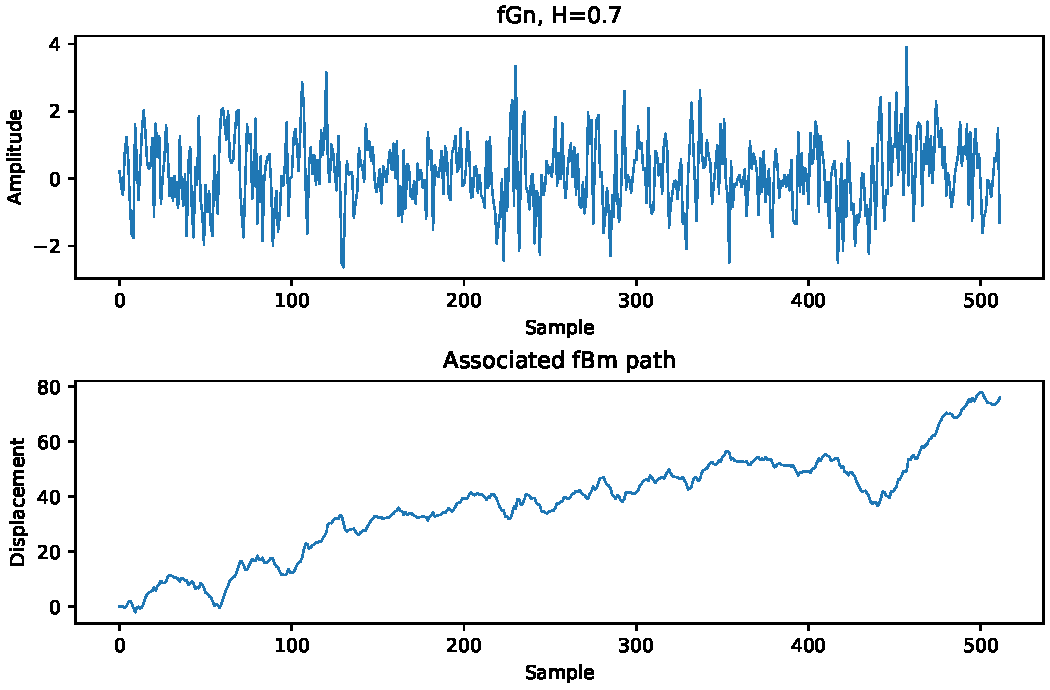
\includegraphics[width=\columnwidth]{figures/signals.pdf}
\caption{A representative Davies--Harte fGn sample and its cumulative fBm path, $H=0.7$, $N=4096$. The plotted portion contains 512 samples.}
\label{fig:signals}
\end{figure}

\begin{figure}[t]
\centering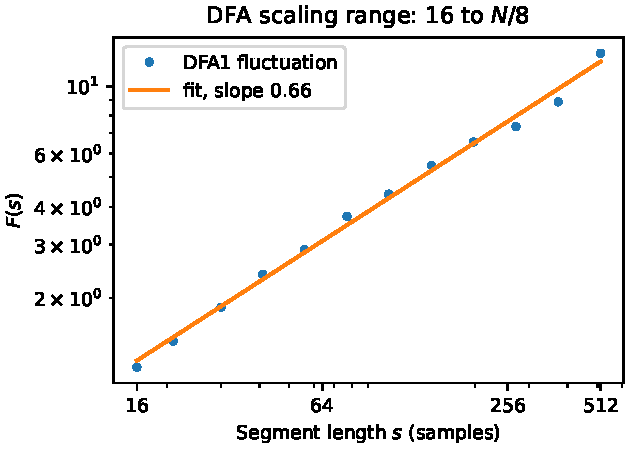
\includegraphics[width=.87\columnwidth]{figures/dfa_scaling.pdf}
\caption{DFA1 fluctuation versus segment length for the same fGn realization. All displayed points from 16 to $N/8$ enter the fitted slope.}
\label{fig:dfa}
\end{figure}

\begin{figure}[t]
\centering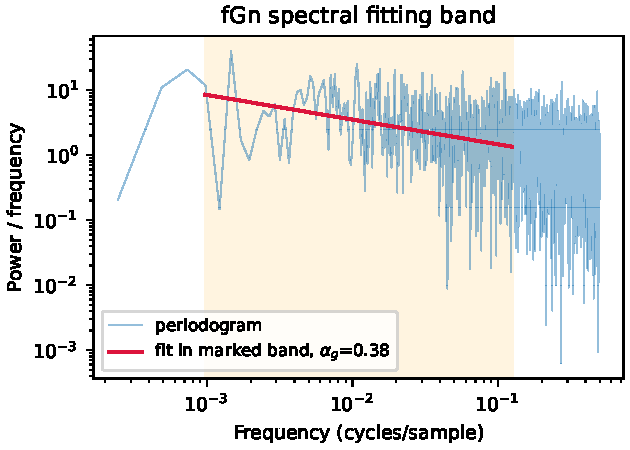
\includegraphics[width=.87\columnwidth]{figures/spectral_fit.pdf}
\caption{Periodogram of the representative fGn sequence. The shaded range is the predetermined low-frequency fitting band; the fitted line illustrates the finite-record spectral slope.}
\label{fig:spectralfit}
\end{figure}

\subsection{Estimator performance on reference processes}

Figure~\ref{fig:hurst} compares three estimates of $H$ and the DFA RMSE as a function of record length. At $N=2^{14}$, $H=0.2$, mean DFA and structure-function estimates are $0.203$ and $0.199$, respectively, whereas R/S gives $0.306$. For $H=0.5$ they are $0.497$, $0.496$, and $0.549$; for $H=0.8$ the corresponding means are $0.797$, $0.775$, and $0.788$. These values do not support a universal ranking of estimators: R/S has a large upward bias at the antipersistent end but much smaller bias for $H=0.8$. Table~\ref{tab:performance} reports bias and RMSE, while the sample standard deviations are retained in \texttt{results/summary.csv}. At $H=0.2$ the R/S standard deviation is only $0.008$, so its RMSE of $0.107$ is dominated by bias. The $H=0.2$ DFA RMSE falls from $0.028$ at $N=2^{10}$ to $0.007$ at $N=2^{16}$, while R/S remains at $0.090$ at the longest length because its bias remains substantial.

\begin{figure*}[t]
\centering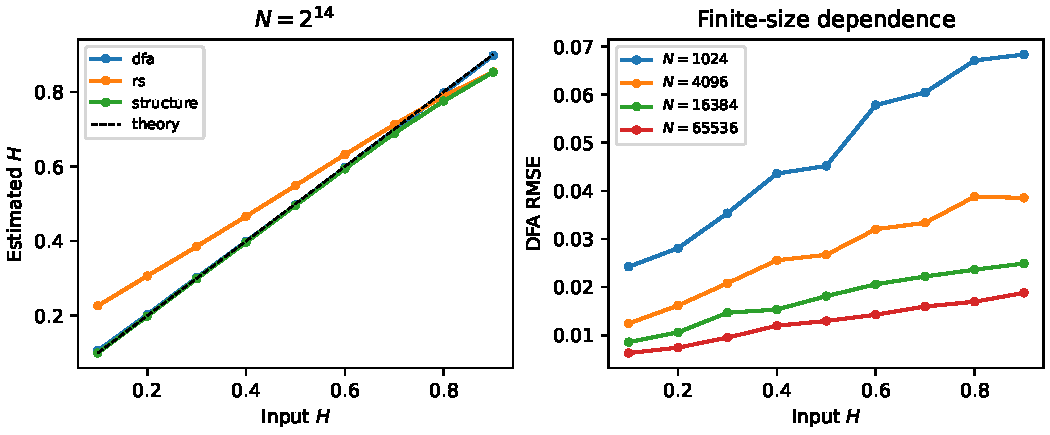
\includegraphics[width=.92\textwidth]{figures/hurst_performance.pdf}
\caption{Mean $H$ estimates at $N=2^{14}$ (left) and DFA RMSE over all four record lengths (right) for exact fGn. Dashed curves indicate the input parameter.}
\label{fig:hurst}
\end{figure*}

\begin{table}[t]
\caption{Selected Davies--Harte results at $N=2^{14}$, with 200 realizations per $H$. Numbers are bias / RMSE relative to the process-specific target; standard deviations are in the saved summary table.}
\label{tab:performance}
\centering\small
\resizebox{\columnwidth}{!}{\begin{tabular}{lccc}
\toprule
Estimator & $H=0.2$ & $H=0.5$ & $H=0.8$\\
\midrule
$H$ from DFA1 & $0.003/0.011$ & $-0.003/0.018$ & $-0.003/0.024$\\
$H$ from R/S & $0.106/0.107$ & $0.049/0.050$ & $-0.012/0.018$\\
$\beta$ from aggregation & $0.003/0.051$ & $0.012/0.052$ & $0.068/0.094$\\
$\alpha_g$ from Welch & $-0.065/0.071$ & $-0.006/0.029$ & $0.005/0.025$\\
$\alpha_w$ from wavelets & $-0.067/0.080$ & $-0.013/0.045$ & $0.001/0.042$\\
$\alpha_B$ from periodogram & $-0.072/0.078$ & $-0.015/0.035$ & $-0.431/0.476$\\
$\alpha_{w,B}$ from wavelets & $-0.081/0.089$ & $-0.019/0.046$ & $-0.009/0.046$\\
$D$ from Higuchi & $0.000/0.007$ & $0.001/0.012$ & $0.001/0.020$\\
$D$ from boxes & $-0.127/0.129$ & $-0.099/0.109$ & $-0.050/0.076$\\
\bottomrule
\end{tabular}}
\end{table}

The ACF and aggregated-variance fits provide distinct estimates of $\beta$. At $N=2^{14}$ and $H=0.6$, the positive-lag ACF fit gives mean $0.523$ and RMSE $0.306$ against the theoretical $0.8$; aggregation gives mean $0.819$ and RMSE $0.061$. At $H=0.8$, their means are $0.556$ and $0.468$ against $0.4$. Selection of positive ACF ordinates and the finite lag range may contribute to the ACF bias in this design. For $H\le1/2$, we report only the aggregated-variance exponent because a positive ACF-tail fit has no intended meaning there.

The spectral, wavelet and geometric estimates appear in Fig.~\ref{fig:spectral}; Fig.~\ref{fig:spectralfit} shows the declared frequency fitting band. At $H=0.2$, Welch and wavelet slopes have biases $-0.065$ and $-0.067$ at $N=2^{14}$, although the nominal fGn spectral exponent is $-0.6$. At $H=0.8$ their biases shrink to $0.005$ and $0.001$. Across the 36 Davies--Harte parameter combinations, mean absolute bias is $0.041$ for Welch and $0.044$ for wavelets, with mean RMSE $0.074$ and $0.087$. The periodogram has lower mean absolute bias ($0.036$) but higher mean RMSE ($0.082$) because its unaveraged ordinates fluctuate more. For Fourier synthesis, mean absolute Welch bias and RMSE are $0.014$ and $0.054$; this generator matches the fitted spectral envelope but does not reproduce the exact fGn covariance.

\begin{figure*}[t]
\centering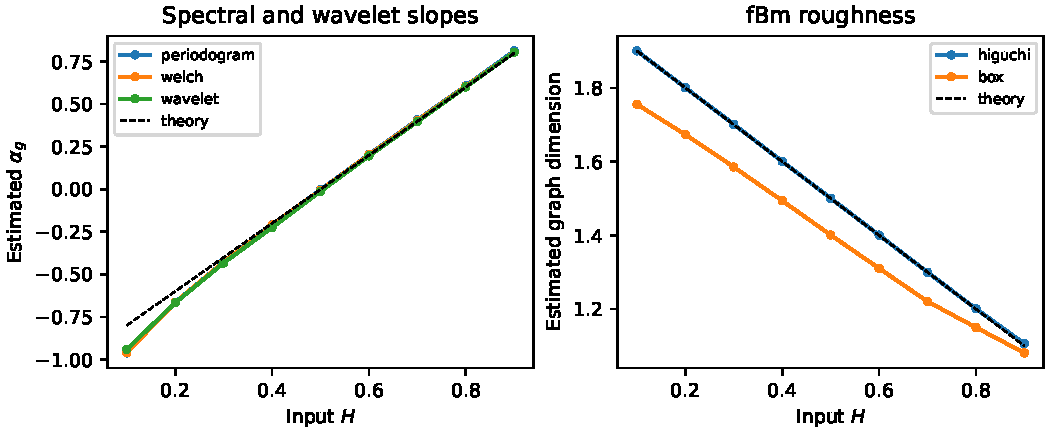
\includegraphics[width=.92\textwidth]{figures/spectral_dimension.pdf}
\caption{Mean fGn spectral and wavelet slopes (left) and fBm graph-dimension estimates (right) at $N=2^{14}$ for Davies--Harte synthesis. Dashed lines are $2H-1$ and $2-H$.}
\label{fig:spectral}
\end{figure*}

\begin{figure*}[t]
\centering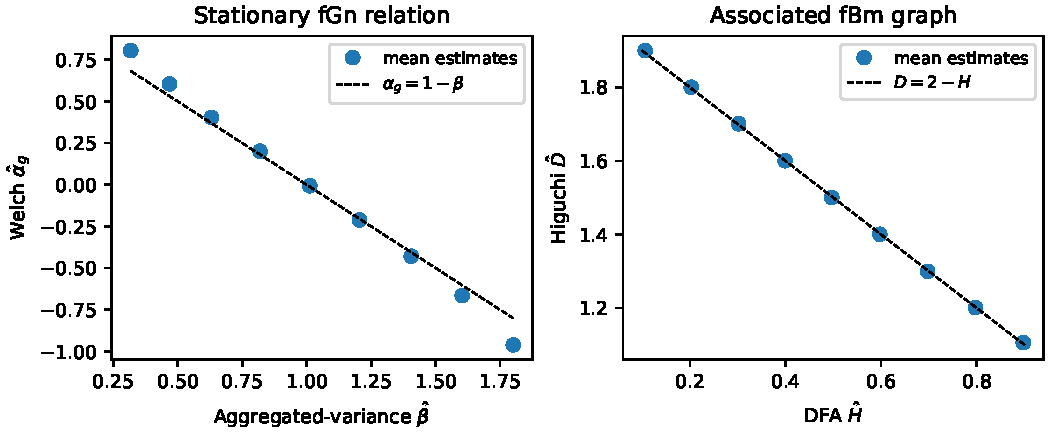
\includegraphics[width=.92\textwidth]{figures/relation_planes.pdf}
\caption{Mean estimates at $N=2^{14}$ paired by their corresponding exponent estimators. The left panel combines the fGn aggregated-variance and Welch estimates; the right panel combines the fGn DFA estimate with the associated fBm Higuchi dimension. Dashed lines are the process-level identities.}
\label{fig:planes}
\end{figure*}

\begin{figure*}[t]
\centering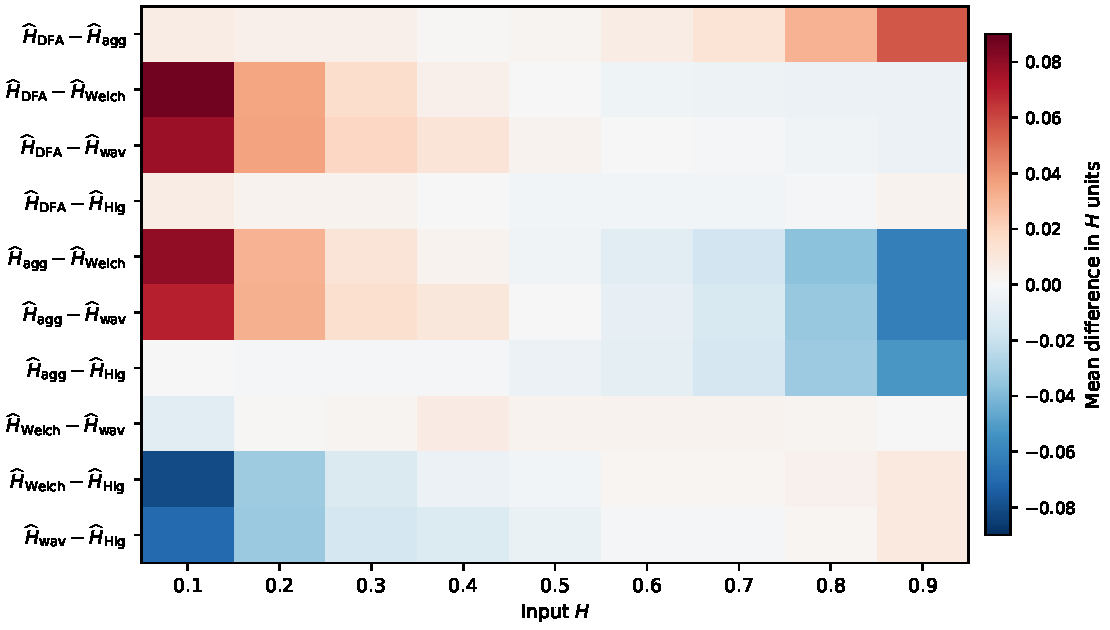
\includegraphics[width=.92\textwidth]{figures/h_discrepancy_heatmap.pdf}
\caption{Mean paired differences among five $H$-equivalent estimators for Davies--Harte fGn and its fBm path at $N=2^{14}$, with 200 realizations for each input $H$. Each row is the first estimator minus the second; the color scale is centered on zero.}
\label{fig:discrepancies}
\end{figure*}

Higuchi's dimension is close to $2-H$ over this grid: mean absolute bias across 36 Davies--Harte parameter combinations is $0.003$, compared with $0.108$ for the finite-grid box count. At $H=0.5$, $N=2^{14}$, the mean estimates are $1.501$ and $1.401$ against $1.5$. The box count increases toward the expected value as the record grows, but its bias remains $-0.089$ at $N=2^{16}$. The normalized ordinate and finite box window influence the measured slope, whereas $D=2-H$ is an asymptotic graph theorem. Estimator bias can therefore create a nonzero residual even for a theoretically correct dimension relation.

For the fBm periodogram, the high-$H$ discrepancy is conspicuous. At $H=0.8$, $N=2^{14}$, its mean fitted slope is $2.169$ while $2H+1=2.6$. The edge-trimmed fBm wavelet estimate has mean $2.591$ and RMSE $0.046$ for the same parameters. Its absolute bias averaged over all 36 Davies--Harte combinations is $0.059$, compared with $0.178$ for the fBm periodogram. The finite path, low-frequency leakage and linear detrending affect the periodogram's operational slope, while wavelet localization and edge removal reduce endpoint influence. At $H=0.2$ the two means are $1.328$ and $1.319$ against $1.4$, so the wavelet advantage is not uniform. The slope $2H+1$ is a finite-path Fourier relation, not a stationary fBm spectral density; direct fitting of the stationary increments gives $\alpha_g$ with smaller bias here.

\subsection{Paired identities and multiplicity}

Across the 36 Davies--Harte parameter combinations, the mean of $\Delta_1$ is $-0.0048$, yet the adjusted $t$ tests reject a zero mean for 24 combinations; Table~\ref{tab:allrelations} also reports 8 for $\Delta_2$ and 19 for $\Delta_3$. These are tests of \emph{finite-sample estimator residuals}, not of the exact process identities. Aggregated variance, Welch and DFA have biases that need not cancel. Higuchi and DFA are close to their targets, giving a mean $\Delta_2$ of only $0.0025$, but 200 paired realizations can resolve small systematic differences. All 576 tests across both generators share one Bonferroni correction.

Figure~\ref{fig:planes} plots the corresponding exponent pairs. Their means follow the expected trends, yet visual agreement does not imply zero paired residuals. Table~\ref{tab:intervals} shows three parameter combinations. At $H=0.2$, $N=2^{14}$, $\Delta_1$ is $-0.0623$ with an unadjusted percentile interval $[-0.0691,-0.0554]$; at $H=0.8$ it is $0.0731$ with interval $[0.0637,0.0823]$. The sign reversal is consistent with finite-band bias in the spectral and aggregated-variance slopes. At $H=0.5$, its interval crosses zero. These 95\% intervals describe uncertainty separately for each mean; the multiplicity correction applies to the $t$-test $p$ values. Thus the $H=0.5$ interval for $\Delta_2$ excludes zero while its adjusted $p$ value is $1.000$.

Figure~\ref{fig:discrepancies} places five estimators on the same $H$ scale: $\widehat H_{\rm DFA}=\widehat\alpha_{\rm DFA}$, $\widehat H_{\rm agg}=1-\widehat\beta_{\rm agg}/2$, $\widehat H_{\rm Welch}=(1+\widehat\alpha_g)/2$, $\widehat H_{\rm wav}=(1+\widehat\alpha_w)/2$, and $\widehat H_{\rm Hig}=2-\widehat D_{\rm Hig}$. For each input $H$, the ten pairwise differences are formed within each realization and then averaged. Color shows the signed disagreement between mean estimates in $H$ units. A nonzero difference can reflect finite-sample bias in either estimator, even when the fGn/fBm identity is exact; the separately specified residual tests address zero means with uncertainty and multiplicity correction. The notebook retains all ten original pairwise scatter plots required by the task.

\begin{table}[t]
\caption{Selected Davies--Harte paired residual means and unadjusted 95\% percentile bootstrap intervals at $N=2^{14}$. Adjusted $p$ values are saved by the notebook.}
\label{tab:intervals}
\centering\small
\begin{tabular}{ccrc}
\toprule
$H$ & Residual & Mean & 95\% interval\\
\midrule
0.2 & $\Delta_1$ & $-0.0623$ & $[-0.0691,-0.0554]$\\
    & $\Delta_2$ & $0.0033$ & $[0.0021,0.0044]$\\
0.5 & $\Delta_1$ & $0.0059$ & $[-0.0017,0.0134]$\\
    & $\Delta_2$ & $-0.0026$ & $[-0.0045,-0.0005]$\\
0.8 & $\Delta_1$ & $0.0731$ & $[0.0637,0.0823]$\\
    & $\Delta_2$ & $-0.0016$ & $[-0.0049,0.0016]$\\
\bottomrule
\end{tabular}
\end{table}

The eight-relation results reveal estimator dependence in algebraically equivalent formulas. For Davies--Harte synthesis, $\widehat D-(5-\widehat\alpha_B)/2$ has mean $-0.0865$ and rejects zero for 31 of 36 parameter combinations, largely because the path periodogram underestimates $\alpha_B$. The simpler $\widehat D-(2-\widehat H)$ has mean $0.0025$ and rejects for 8. The mean fBm wavelet-minus-periodogram slope is $0.1183$, whereas the fGn wavelet-minus-Welch mean is $-0.0006$. This near-zero aggregate hides differences among parameter combinations: 13 still reject after correction. Intervals and adjusted $p$ values for each combination are in \texttt{results/all\_relations.csv}.

\begin{table}[t]
\caption{Eight paired identities for Davies--Harte synthesis: mean residual across 36 parameter combinations and number rejecting zero after Bonferroni correction over 576 tests. Each residual is the left side minus the right side.}
\label{tab:allrelations}
\centering\small
\resizebox{\columnwidth}{!}{\begin{tabular}{lrr}
\toprule
Identity & Mean residual & Rejections\\
\midrule
$\beta=2-2H$ & $0.0350$ & $19/36$\\
$\alpha_g=1-\beta$ & $-0.0048$ & $24/36$\\
$\alpha_B=\alpha_g+2$ & $-0.1382$ & $22/36$\\
$D=2-H$ & $0.0025$ & $8/36$\\
$D=(5-\alpha_B)/2$ & $-0.0865$ & $31/36$\\
$D=1+\beta/2$ & $-0.0150$ & $14/36$\\
$\alpha_{w,g}=\alpha_g$ & $-0.0006$ & $13/36$\\
$\alpha_{w,B}=\alpha_B$ & $0.1183$ & $29/36$\\
\bottomrule
\end{tabular}}
\end{table}

\subsection{Controlled departures from scale invariance}

Figure~\ref{fig:contrasts} shows mean DFA1 fluctuation curves from the 200 realizations of each representative signal at $N=4096$. Each curve is divided by its own realization's $F(16)$ before averaging, so its shape can be compared without amplitude differences. The exact fGn reference is nearly straight over the fitted scales; the periodic signal bends markedly near its 128-sample period. Its single fitted DFA slope is $0.837$, compared with $0.697$ for the reference. White-noise addition lowers mean DFA to $0.672$. At this length the linear trend shifts DFA only to $0.709$, although its accumulated-path structure estimate rises to $0.870$ and Higuchi dimension falls to $1.035$. DFA1 removes constant trends in the original series, not a linear trend, which becomes quadratic in its integrated profile; DFA2 would be needed for that removal \cite{kantelhardt2002}.

The Lorentzian-mixture signal has a mean Welch slope $0.973$ and DFA slope $0.945$ in the selected bands. Both are close to its interior $1/f$ regime, but its spectrum levels off below the lowest relaxation rate; no global fGn $H=0.7$ applies. For the Cauchy signal, aggregated variance gives mean $\widehat\beta=0.433$ and an operational $\widehat H=1-\widehat\beta/2=0.784$, near its specified large-lag $0.75$. The integer-lag structure slope on the stationary Cauchy values is $0.083$, and Higuchi's dimension is $1.922$. Neither recovers the continuous small-lag targets $H_{\rm loc}=0.35$ and $D=1.65$: the sampling interval cannot approach zero. These estimates illustrate the scale separation but do not numerically establish the theoretical local dimension.

Table~\ref{tab:contrasts} records the corresponding means. DFA and Welch are applied to each raw input, whereas structure and Higuchi use cumulative paths in the first five rows and the stationary Cauchy values in the last. The latter two columns thus describe local behavior of different mathematical objects; their Cauchy entries are not estimates of the same fBm path parameter as the other rows. No common true exponent exists for the cutoff or contaminated signals, so we do not label their departures from $0.7$ as estimator bias. Their realization-level estimates, from which standard deviations can be calculated, are saved in \texttt{results/contrasts.csv}.

\begin{table}[t]
\caption{Mean estimates for the six contrast processes at $N=4096$; 200 realizations per process. The Cauchy graph and structure statistics use the stationary process directly.}
\label{tab:contrasts}
\centering\small
\resizebox{\columnwidth}{!}{\begin{tabular}{lrrrr}
\toprule
Process & DFA & Structure & Welch & Higuchi\\
\midrule
Exact fGn reference & 0.697 & 0.685 & 0.391 & 1.302\\
Additive white noise & 0.672 & 0.660 & 0.332 & 1.326\\
Linear trend & 0.709 & 0.870 & 0.391 & 1.035\\
Periodic component & 0.837 & 0.718 & 0.523 & 1.179\\
Lorentzian $1/f$ cutoff & 0.945 & 0.850 & 0.973 & 1.142\\
Generalized Cauchy & 0.862 & 0.083 & 0.775 & 1.922\\
\bottomrule
\end{tabular}}
\end{table}

\begin{figure*}[t]
\centering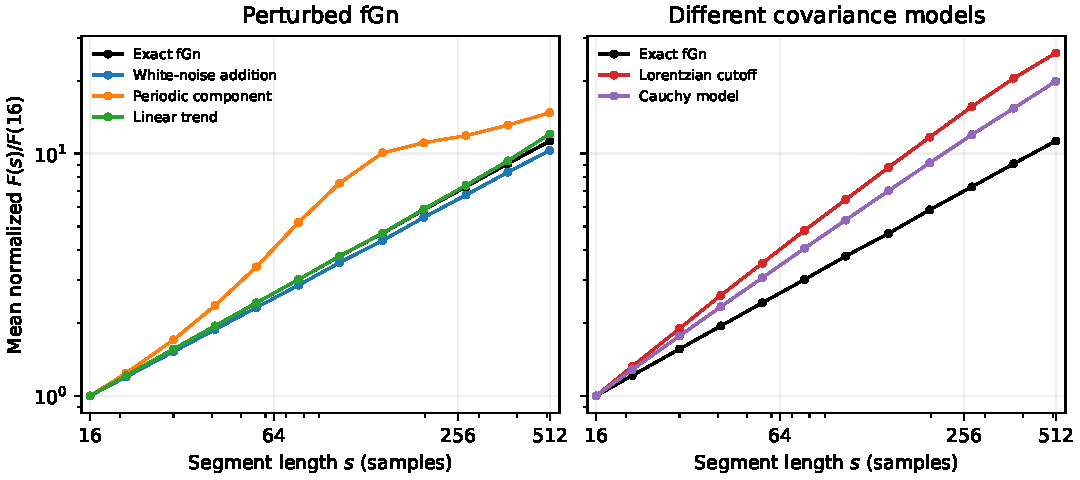
\includegraphics[width=.93\textwidth]{figures/contrasts.pdf}
\caption{Mean normalized DFA1 fluctuation curves for the representative contrasts ($N=4096$). Each realization contributes $F(s)/F(16)$ before averaging; all 12 displayed scales from 16 to 512 enter the individual slope fits. The same DFA procedure is applied to each raw input.}
\label{fig:contrasts}
\end{figure*}

The extended contrast grid adds 28,800 realizations: four parameterized perturbations at nine $H$ values and four $N$ values, with 200 repetitions per combination. At the baseline or global parameter $H=0.7$, the fixed linear trend raises mean DFA1 from $0.700$ at $N=2^{10}$ to $1.057$ at $N=2^{16}$ because its accumulated deterministic component grows with record length. The periodic component instead falls from $1.133$ to $0.651$ as its fixed 128-sample period occupies a smaller share of the fitted scale range. Additive noise changes the mean only from $0.661$ to $0.680$. The integer-grid Cauchy DFA mean falls from $0.848$ to $0.791$, while its Higuchi dimension remains near $1.93$. These results remain available in \texttt{results/contrast\_grid.csv}; no separate length plot is needed.

The Cauchy graph estimator uses steps 2 to 64 and cannot access the $k\to0$ limit. Also, the bootstrap intervals above quantify uncertainty in the reference-process residual means; they were not computed for contrasts and should not be read as uncertainty bounds on the contrast effects. The original task's suggested robustness ranking is therefore evaluated through the measured reference biases and contrast behavior, not assumed in advance.

\section{Conclusions}

The numerical results support the process-specific scaling conventions while showing that a finite-sample relation residual can be driven by the estimators used to construct it. DFA1 and a structure function recover $H$ accurately for exact fGn/fBm over much of the tested grid, whereas R/S has pronounced upward bias for antipersistent short records. Higuchi's local graph dimension tracks $2-H$ closely in the exact fBm simulations; the chosen finite-grid box count underestimates it. Spectral and wavelet estimates are sensitive to fitting bands, especially for antipersistent fGn. At high $H$, the edge-trimmed fBm wavelet slope is much closer to $2H+1$ than the raw fBm periodogram slope in this design.

The mathematical distinction is essential: $\beta$ describes the fGn covariance tail, $\alpha_g$ its stationary spectral density, and $D$ the roughness of the associated fBm graph. Their combined equalities cannot simply be assigned to an arbitrary stationary series or to a Cauchy process with independent local and global scaling. Additive noise, trends, periodicities and spectral cutoffs further change observed slopes across the finite ranges used in practice. The saved notebook outputs permit the choices of generator, estimator and fitting window to be re-examined without treating any single observed power-law segment as universal.

\bibliographystyle{unsrt}
\bibliography{references}
\end{document}
